\documentclass[12pt,a4paper]{article}

\usepackage[utf8]{inputenc}
\usepackage[T1]{fontenc}
\usepackage{geometry}
\usepackage{titlesec}
\usepackage{enumitem}
\usepackage{hyperref}
\usepackage{parskip}
\usepackage{amsmath}
\usepackage{graphicx}
\usepackage{float}
\graphicspath{{img/}}
\usepackage{tikz}
\usepackage{tikz-timing}
\usetikzlibrary{arrows.meta, decorations.markings, fit, positioning}

\geometry{margin=2.5cm}

\hypersetup{
    colorlinks=true,
    linkcolor=blue,
    urlcolor=blue
}

\begin{document}

\begin{titlepage}
    \centering
    \vspace*{\fill}
    {\Huge\textbf{Autonomous Driving Vehicle}}
    \vspace*{\fill}
\end{titlepage}

\tableofcontents
\newpage

% ============================================================
\section{Hardware}

\subsection*{Vehicle Platform}

% ---- STM32F401 NUCLEO ----
\subsubsection*{STM32F401 NUCLEO}

\begin{figure}[H]
\centering
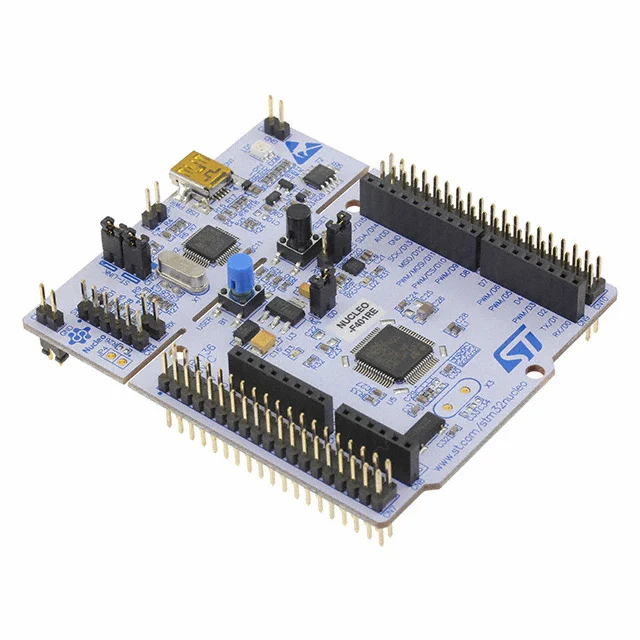
\includegraphics[width=0.45\textwidth]{NUCLEO-F401RE.png}
\caption{STM32F401 NUCLEO board}
\end{figure}

\begin{table}[H]
\centering
\begin{tabular}{ll}
\hline
\textbf{Property} & \textbf{Value} \\
\hline
MCU        & STM32F401RE (ARM Cortex-M4) \\
Clock      & Up to 84\,MHz \\
Flash      & 512\,KB \\
RAM        & 96\,KB \\
Interface  & UART, I2C, SPI, GPIO, ADC, PWM \\
Role       & Low-level control: motor, servo, sensor reading \\
\hline
\end{tabular}
\caption{STM32F401 NUCLEO specifications}
\end{table}

% ---- Raspberry Pi 5 ----
\subsubsection*{Raspberry Pi 5}

\begin{figure}[H]
\centering
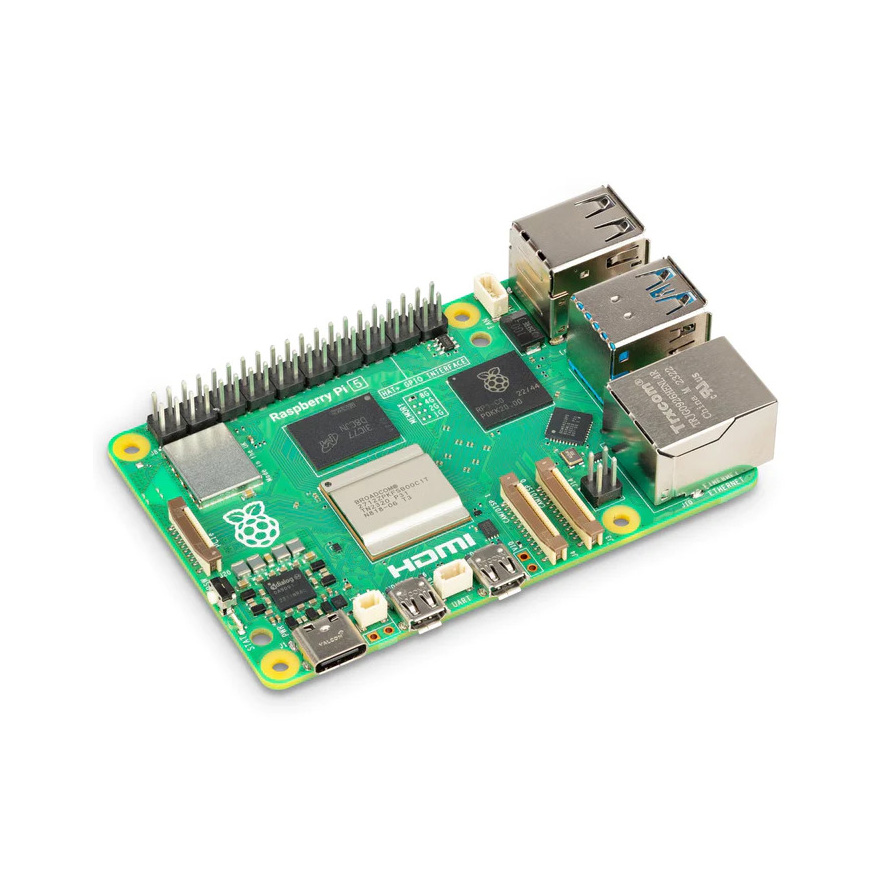
\includegraphics[width=0.45\textwidth]{raspberry-pi-5}
\caption{Raspberry Pi 5}
\end{figure}

\begin{table}[H]
\centering
\begin{tabular}{ll}
\hline
\textbf{Property} & \textbf{Value} \\
\hline
CPU        & Broadcom BCM2712, quad-core Cortex-A76 @ 2.4\,GHz \\
RAM        & 4\,GB / 8\,GB LPDDR4X \\
OS         & Ubuntu 24.04 (64-bit) \\
Interface  & UART, USB, CSI camera, Ethernet, Wi-Fi \\
Role       & High-level brain: perception, planning, control \\
\hline
\end{tabular}
\caption{Raspberry Pi 5 specifications}
\end{table}

% ---- AS5600 ----
\subsubsection*{Encoder: AS5600}

\begin{figure}[H]
\centering
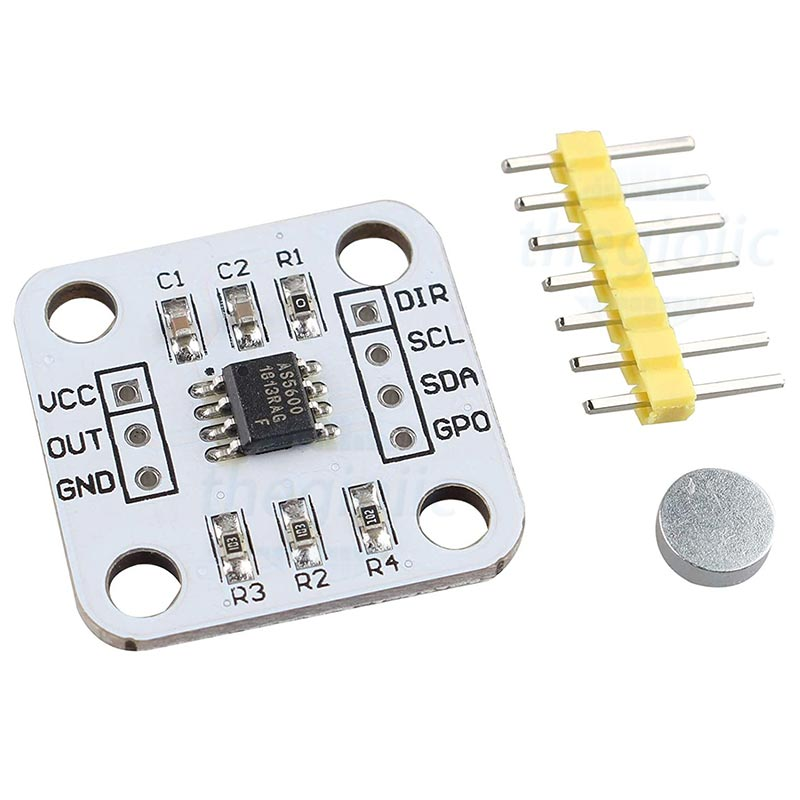
\includegraphics[width=0.4\textwidth]{AS5600}
\caption{AS5600 magnetic rotary encoder module}
\end{figure}

\begin{table}[H]
\centering
\begin{tabular}{ll}
\hline
\textbf{Property} & \textbf{Value} \\
\hline
Type           & Contactless magnetic rotary encoder \\
Resolution     & 12-bit (4096 positions/revolution) \\
Interface      & I2C (address 0x36) \\
Supply voltage & 3.3\,V -- 5\,V \\
Output         & Absolute angle 0°--360° \\
Role           & Measures wheel rotation for speed estimation \\
\hline
\end{tabular}
\caption{AS5600 encoder specifications}
\end{table}

% ---- BNO055 ----
\subsubsection*{IMU: BNO055}

\begin{figure}[H]
\centering
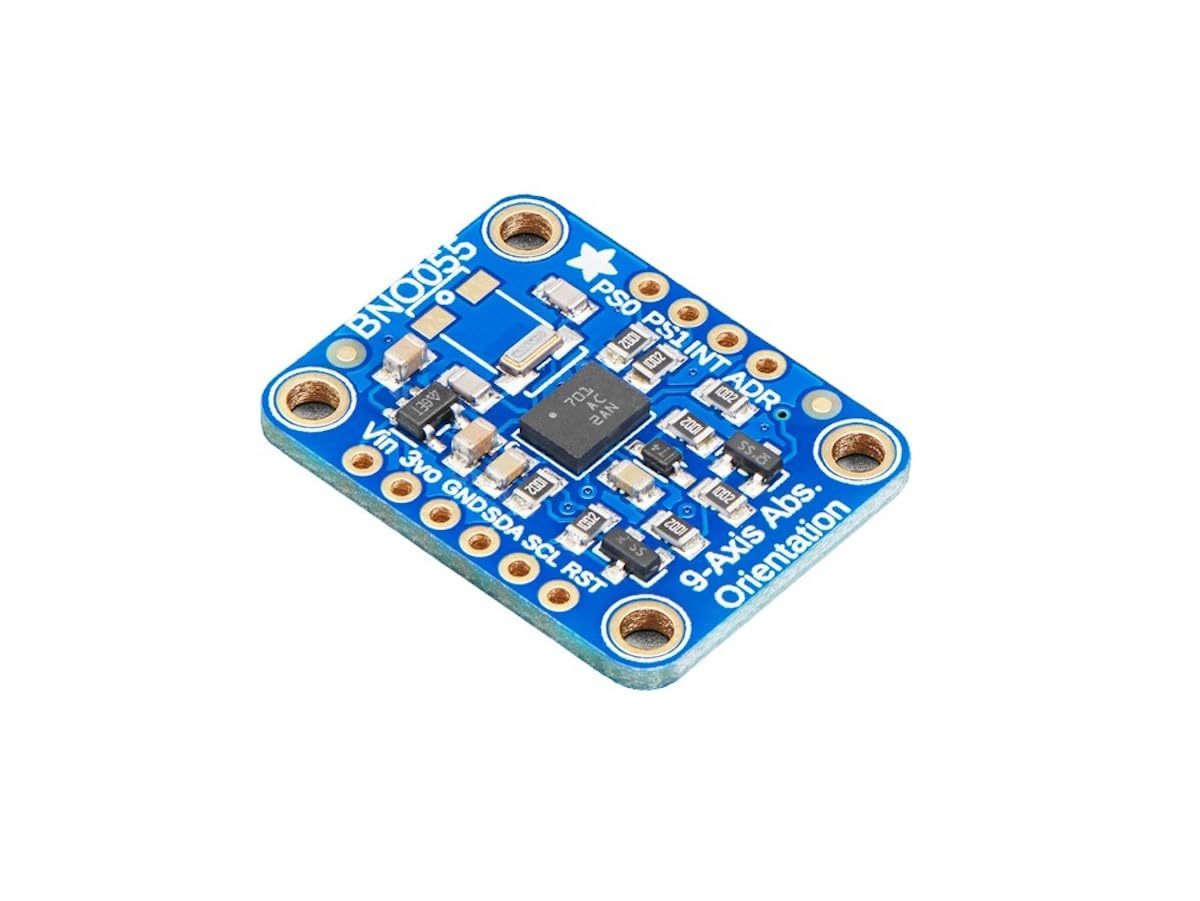
\includegraphics[width=0.4\textwidth]{BNO055}
\caption{BNO055 9-axis IMU module}
\end{figure}

\begin{table}[H]
\centering
\begin{tabular}{ll}
\hline
\textbf{Property} & \textbf{Value} \\
\hline
Axes           & 9-axis (accelerometer + gyroscope + magnetometer) \\
Interface      & I2C (address 0x28 / 0x29) \\
Output         & Euler angles: yaw, pitch, roll (degrees) \\
Supply voltage & 3.3\,V \\
Fusion mode    & NDOF (on-chip sensor fusion) \\
Role           & Provides heading angle (yaw) for state estimation \\
\hline
\end{tabular}
\caption{BNO055 IMU specifications}
\end{table}

% ---- Servo ----
\subsubsection*{Actuator: Steering Servo}

\begin{figure}[H]
\centering
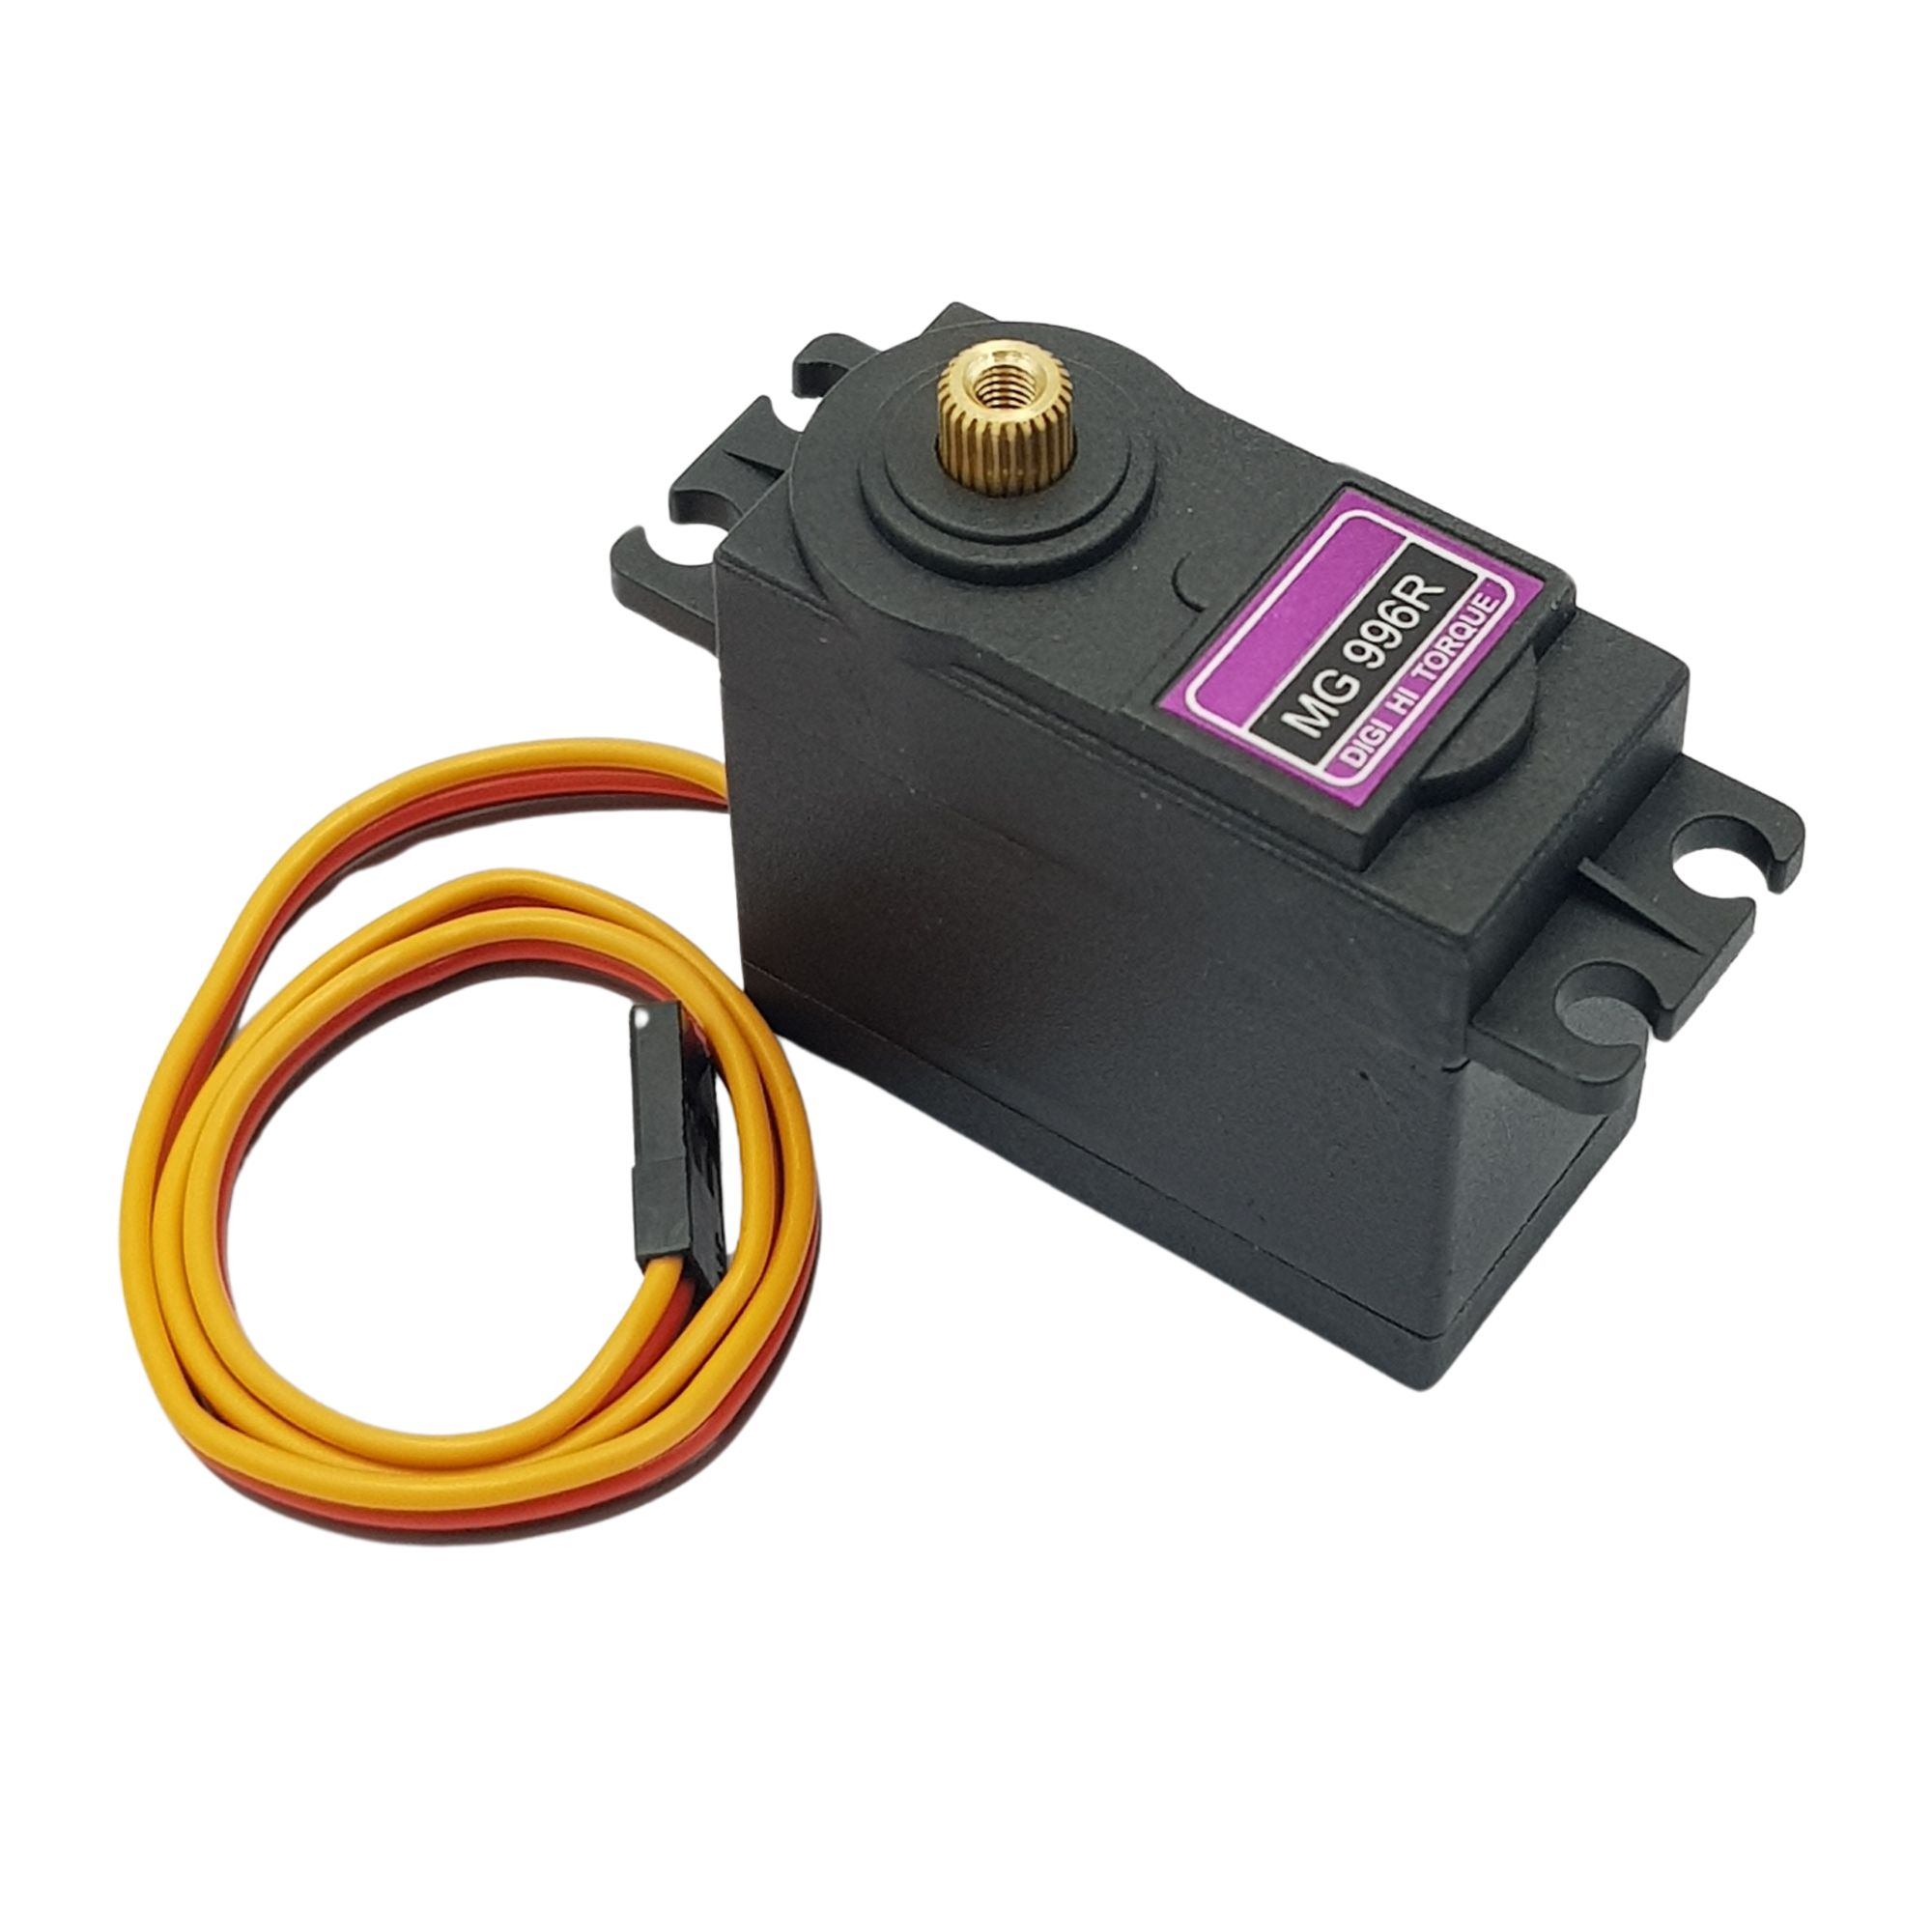
\includegraphics[width=0.4\textwidth]{Angle-ServoServo}
\caption{180° steering servo}
\end{figure}

\begin{table}[H]
\centering
\begin{tabular}{ll}
\hline
\textbf{Property} & \textbf{Value} \\
\hline
Type           & PWM position servo \\
Range          & 0°--180° \\
Control        & PWM 50\,Hz, pulse width 1--2\,ms \\
Supply voltage & 5\,V \\
Role           & Controls front wheel steering angle \\
\hline
\end{tabular}
\caption{Steering servo specifications}
\end{table}

\subsection*{Simulator}
\begin{itemize}
    \item Encoder: AS5600
    \item Motor
    \item 3D Model design
\end{itemize}

% ============================================================
\section{Software}

\subsection{Architecture}

% ------ Embedded Platform ------
\subsubsection{Embedded Platform}

\begin{figure}[H]
\centering
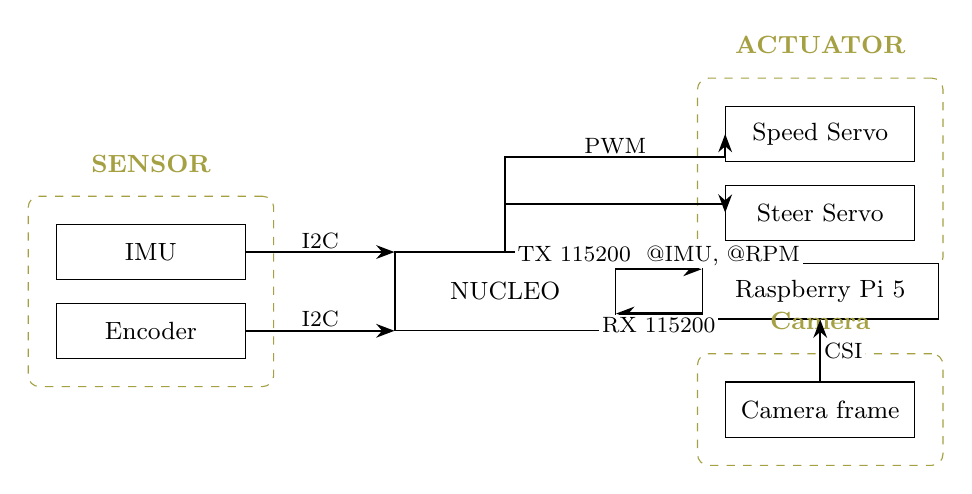
\begin{tikzpicture}[
  node/.style={draw, fill=white, minimum width=2.4cm, minimum height=0.7cm,
               font=\small, align=center},
  group/.style={draw, dashed, rounded corners, yellow!60!black, inner sep=10pt},
  grplbl/.style={font=\small\bfseries, yellow!60!black},
  arr/.style={-{Stealth}, thick},
  lbl/.style={font=\footnotesize, fill=white, inner sep=1pt}
]

%
%  Layout (grid):
%
%  row  3 :                    [Speed Servo]
%  row  2 :                    [Steer Servo]    ACTUATOR
%  row  1 :  [IMU]     [NUCLEO]              [Raspberry Pi 5]
%  row  0 :  [Encoder]
%  row -1 :                    [Camera frame]   Camera
%
%  col:  0         3           6              9

% --- SENSOR ---
\node[node] (imu)     at (0,  1.0) {IMU};
\node[node] (encoder) at (0,  0.0) {Encoder};
\node[group, fit=(imu)(encoder)] (sen_box) {};
\node[grplbl, above=5pt of sen_box] {SENSOR};

% --- NUCLEO ---
\node[node, minimum width=2.8cm, minimum height=1.0cm]
      (nucleo) at (4.5, 0.5) {NUCLEO};

% --- ACTUATOR ---
\node[node] (speed) at (8.5, 2.5) {Speed Servo};
\node[node] (steer) at (8.5, 1.5) {Steer Servo};
\node[group, fit=(speed)(steer)] (act_box) {};
\node[grplbl, above=5pt of act_box] {ACTUATOR};

% --- Raspberry Pi 5 ---
\node[node, minimum width=3.0cm] (rpi) at (8.5, 0.5) {Raspberry Pi 5};

% --- Camera ---
\node[node] (camera) at (8.5, -1.0) {Camera frame};
\node[group, fit=(camera)] (cam_box) {};
\node[grplbl, above=5pt of cam_box] {Camera};

% ---- Connections ----

% IMU → NUCLEO (I2C), top wire
\draw[arr] (imu.east) -- node[lbl, above] {I2C} (nucleo.west |- imu);

% Encoder → NUCLEO (I2C), bottom wire
\draw[arr] (encoder.east) -- node[lbl, above] {I2C} (nucleo.west |- encoder);

% NUCLEO → Speed Servo (PWM)
\draw[arr] (nucleo.north) -- ++(0, 1.2) -| node[lbl, pos=0.25, above] {PWM} (speed.west);

% NUCLEO → Steer Servo (PWM)
\draw[arr] (nucleo.north) -- ++(0, 0.6) -| (steer.west);

% NUCLEO → RPi TX (UART)
\draw[arr] ([yshift= 8pt]nucleo.east) -- node[lbl, above] {TX 115200 \ @IMU, @RPM}
           ([yshift= 8pt]rpi.west);

% RPi → NUCLEO RX (UART)
\draw[arr] ([yshift=-8pt]rpi.west) -- node[lbl, below] {RX 115200}
           ([yshift=-8pt]nucleo.east);

% Camera → RPi (CSI)
\draw[arr] (camera.north) -- node[lbl, right] {CSI} (rpi.south);

\end{tikzpicture}
\caption{Embedded Platform: NUCLEO reads sensors (I2C), drives actuators (PWM), communicates with Raspberry Pi 5 via UART}
\end{figure}

% ------ Brain ------
\subsubsection{Brain}

\begin{figure}[H]
\centering
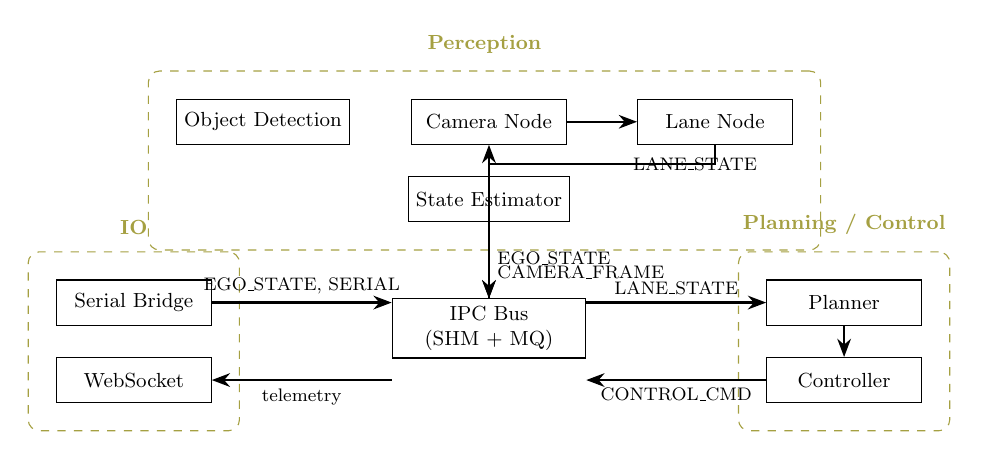
\begin{tikzpicture}[scale=0.82, every node/.style={transform shape},
  node/.style={draw, fill=white, minimum width=2.4cm, minimum height=0.7cm,
               font=\small, align=center},
  group/.style={draw, dashed, rounded corners, inner sep=10pt},
  arr/.style={-{Stealth}, thick},
  lbl/.style={font=\footnotesize}
]

% IO layer (left)
\node[node] (serial)  at (-5.5,  0.4) {Serial Bridge};
\node[node] (ws)      at (-5.5, -0.8) {WebSocket};
\node[group, yellow!60!black, fit=(serial)(ws)] (io_box) {};
\node[above=4pt of io_box, font=\small\bfseries, yellow!60!black] {IO};

% IPC bus (center)
\node[node, minimum width=3.0cm] (ipc) at (0, 0) {IPC Bus\\(SHM + MQ)};

% Perception layer (top)
\node[node] (cam_node)  at ( 0.0,  3.2) {Camera Node};
\node[node] (lane)      at ( 3.5,  3.2) {Lane Node};
\node[node] (od)        at (-3.5,  3.2) {Object Detection};
\node[node] (state)     at ( 0.0,  2.0) {State Estimator};
\node[group, yellow!60!black, fit=(cam_node)(lane)(od)(state)] (perc_box) {};
\node[above=4pt of perc_box, font=\small\bfseries, yellow!60!black] {Perception};

% Planning (right)
\node[node] (plan) at (5.5, 0.4) {Planner};

% Control (right bottom)
\node[node] (ctrl) at (5.5, -0.8) {Controller};

\node[group, yellow!60!black, fit=(plan)(ctrl)] (brain_box) {};
\node[above=4pt of brain_box, font=\small\bfseries, yellow!60!black] {Planning / Control};

% Arrows
% Serial Bridge ↔ IPC
\draw[arr] (serial.east) -- (ipc.west |- serial)
  node[midway, above, lbl] {EGO\_STATE, SERIAL};
% WebSocket ↔ IPC
\draw[arr] (ipc.west |- ws) -- (ws.east)
  node[midway, below, lbl] {telemetry};

% Perception ↔ IPC
\draw[arr] (ipc.north) -- ++(0,0.4) -| (cam_node.south)
  node[pos=0.3, right, lbl] {CAMERA\_FRAME};
\draw[arr] (cam_node.east) -- (lane.west)
  node[midway, above, lbl] {};
\draw[arr] (state.south) -- (ipc.north |- state) -- (ipc.north)
  node[pos=0.6, right, lbl] {EGO\_STATE};
\draw[arr] (lane.south) -- ++(0,-0.3) -| (ipc.north)
  node[pos=0.2, right, lbl] {LANE\_STATE};

% Planning ↔ IPC
\draw[arr] (ipc.east |- plan) -- (plan.west)
  node[midway, above, lbl] {LANE\_STATE};
\draw[arr] (plan.south) -- (ctrl.north)
  node[midway, right, lbl] {};
\draw[arr] (ctrl.west) -- (ipc.east |- ctrl)
  node[midway, below, lbl] {CONTROL\_CMD};

\end{tikzpicture}
\caption{Brain architecture: nodes communicate via IPC bus (SHM for latest-wins, MQ for queued messages)}
\end{figure}

% ------------------------------------------------------------
\subsection{Embedded Platform}

\subsubsection{Peripheral}

% ---- I2C ----
\textbf{I2C (Inter-Integrated Circuit)}

I2C is a two-wire synchronous serial protocol using a shared clock line (SCL) and a bidirectional data line (SDA).
Communication is initiated by a START condition (SDA falls while SCL is high), followed by a 7-bit device address,
a read/write bit, an ACK from the slave, data bytes, and a STOP condition (SDA rises while SCL is high).
In this project, I2C is used to communicate with the BNO055 IMU at address \texttt{0x28}.

\begin{figure}[h]
\centering
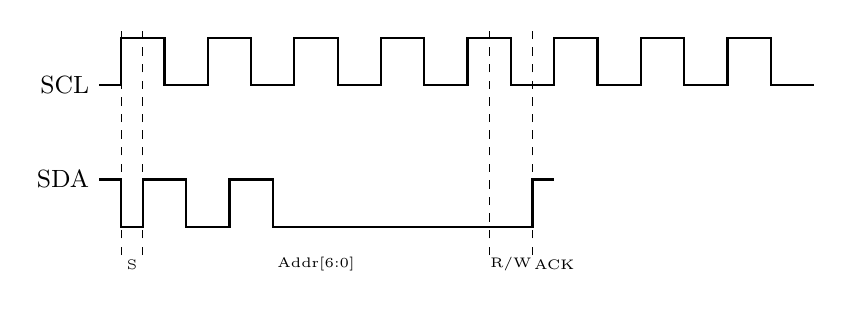
\begin{tikzpicture}[x=0.55cm, y=0.6cm,
    bus/.style={draw, fill=gray!20}]
  % SCL
  \draw[thick] (0,2) node[left]{\small SCL}
    -- ++(0.5,0) -- ++(0,1) -- ++(1,0) -- ++(0,-1)
    -- ++(1,0) -- ++(0,1) -- ++(1,0) -- ++(0,-1)
    -- ++(1,0) -- ++(0,1) -- ++(1,0) -- ++(0,-1)
    -- ++(1,0) -- ++(0,1) -- ++(1,0) -- ++(0,-1)
    -- ++(1,0) -- ++(0,1) -- ++(1,0) -- ++(0,-1)
    -- ++(1,0) -- ++(0,1) -- ++(1,0) -- ++(0,-1)
    -- ++(1,0) -- ++(0,1) -- ++(1,0) -- ++(0,-1)
    -- ++(1,0) -- ++(0,1) -- ++(1,0) -- ++(0,-1)
    -- ++(1,0);
  % SDA — START | A6 A5 A4 A3 A2 A1 A0 | R/W | ACK | STOP
  \draw[thick] (0,0) node[left]{\small SDA}
    -- ++(0.5,0)
    -- ++(0,-1) % START: SDA falls (SCL high region before first clock)
    -- ++(0.5,0)
    % A6=1
    -- ++(0,1) -- ++(1,0)
    % A5=0
    -- ++(0,-1) -- ++(1,0)
    % A4=1
    -- ++(0,1) -- ++(1,0)
    % A3=0
    -- ++(0,-1) -- ++(1,0)
    % A2=0
    -- ++(0,0) -- ++(1,0)
    % A1=0
    -- ++(0,0) -- ++(1,0)
    % A0=0 (0x28 = 0b0101000)
    -- ++(0,0) -- ++(1,0)
    % R/W=0 (write)
    -- ++(0,0) -- ++(1,0)
    % ACK (slave pulls low)
    -- ++(0,0) -- ++(1,0)
    % STOP: SDA rises
    -- ++(0,1) -- ++(0.5,0);
  % Labels
  \draw[dashed] (0.5, -1.6) -- (0.5, 3.2);
  \draw[dashed] (1.0, -1.6) -- (1.0, 3.2);
  \draw[dashed] (9.0, -1.6) -- (9.0, 3.2);
  \draw[dashed] (10.0,-1.6) -- (10.0,3.2);
  \node at (0.75,-1.8) {\tiny S};
  \node at (5.0, -1.8) {\tiny Addr[6:0]};
  \node at (9.5, -1.8) {\tiny R/W};
  \node at (10.5,-1.8) {\tiny ACK};
\end{tikzpicture}
\caption{I2C transaction: START, 7-bit address (0x28), R/W bit, ACK}
\end{figure}

% ---- PWM ----
\textbf{PWM (Pulse Width Modulation)}

PWM generates a periodic digital signal with fixed frequency and variable duty cycle.
The STM32 timer compares the counter value against a capture/compare register (CCR);
output is high when \texttt{CNT < CCR} and low otherwise.
PWM is used to control the servo steering angle and to send throttle commands to the ESC.
Typical servo period is 20\,ms (50\,Hz); pulse width 1--2\,ms maps to 0°--180°.

\begin{figure}[h]
\centering
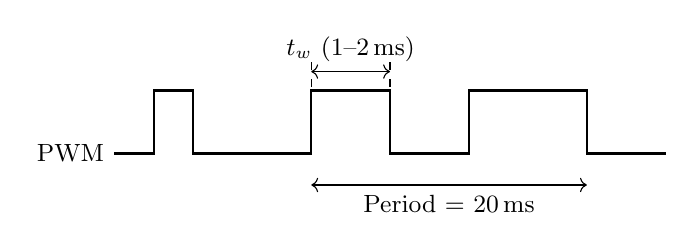
\begin{tikzpicture}[x=1.0cm, y=0.8cm]
  \draw[thick] (0,0) node[left]{\small PWM}
    -- ++(0.5,0) -- ++(0,1) -- ++(0.5,0) -- ++(0,-1)  % pulse 1 (short)
    -- ++(1.5,0) -- ++(0,1) -- ++(1.0,0) -- ++(0,-1)  % pulse 2 (medium)
    -- ++(1.0,0) -- ++(0,1) -- ++(1.5,0) -- ++(0,-1)  % pulse 3 (wide)
    -- ++(1.0,0);
  % Period brace for pulse 2
  \draw[<->] (2.5,-0.5) -- ++(3.5,0) node[midway, below]{\small Period = 20\,ms};
  % Width brace
  \draw[<->] (2.5,1.3) -- ++(1.0,0) node[midway, above]{\small $t_w$ (1--2\,ms)};
  \draw[dashed] (2.5,0) -- (2.5,1.5);
  \draw[dashed] (3.5,0) -- (3.5,1.5);
\end{tikzpicture}
\caption{PWM signal: varying pulse width, fixed 50\,Hz period}
\end{figure}

% ---- UART ----
\textbf{UART (Universal Asynchronous Receiver/Transmitter)}

UART is an asynchronous serial protocol with no shared clock.
A frame consists of: 1 start bit (low), 8 data bits (LSB first), optional parity, and 1--2 stop bits (high).
Both ends must agree on the same baud rate. This project uses 115200\,baud, 8N1 (no parity, 1 stop bit).
The STM32 transmits sensor data to the Raspberry Pi 5 over UART in ASCII frames:
\texttt{@IMU:yaw,pitch,roll;;\textbackslash r\textbackslash n} and \texttt{@RPM:rpm;;\textbackslash r\textbackslash n}.

\begin{figure}[h]
\centering
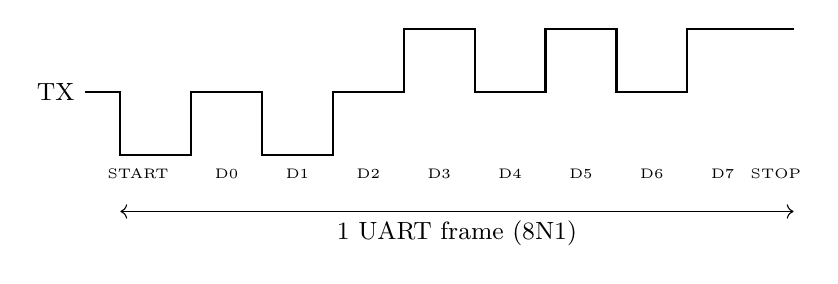
\begin{tikzpicture}[x=0.9cm, y=0.8cm]
  \draw[thick] (0,1) node[left]{\small TX}
    -- ++(0.5,0)          % idle high
    -- ++(0,-1)           % START bit
    -- ++(1,0)            % D0
    -- ++(0,1) -- ++(1,0) % D1
    -- ++(0,-1)-- ++(1,0) % D2
    -- ++(0,1) -- ++(1,0) % D3
    -- ++(0,1) -- ++(1,0) % D4 (high)
    -- ++(0,-1)-- ++(1,0) % D5
    -- ++(0,1) -- ++(1,0) % D6
    -- ++(0,-1)-- ++(1,0) % D7
    -- ++(0,1) -- ++(1,0) % STOP
    -- ++(0.5,0);         % idle
  % Annotations
  \node at (0.75, -0.3) {\tiny START};
  \foreach \i/\b in {1/0, 2/1, 3/0, 4/1, 5/1, 6/0, 7/1, 8/0} {
    \node at (\i+1.0, -0.3) {\tiny D\the\numexpr\i-1\relax};
  }
  \node at (9.75, -0.3) {\tiny STOP};
  \draw[<->] (0.5,-0.9) -- ++(9.5,0) node[midway, below]{\small 1 UART frame (8N1)};
\end{tikzpicture}
\caption{UART frame: start bit, 8 data bits (LSB first), stop bit}
\end{figure}

% ---- RCC ----
\textbf{RCC (Reset and Clock Control)}

The RCC peripheral on the STM32F401 manages system clock configuration and peripheral clock gating.
The internal HSI oscillator (16\,MHz) or external HSE crystal can be fed into the PLL to generate
the system clock (SYSCLK). On the STM32F401 NUCLEO, SYSCLK is configured to 84\,MHz.
Peripheral buses APB1 (max 42\,MHz) and APB2 (max 84\,MHz) are derived via prescalers.
Each peripheral must have its bus clock explicitly enabled via \texttt{RCC\_APBxENR} before use.

\begin{figure}[h]
\centering
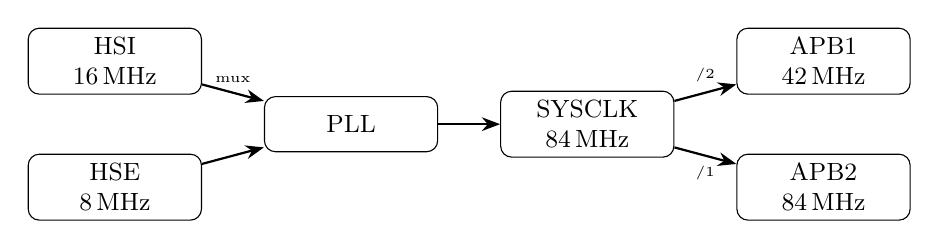
\begin{tikzpicture}[
  box/.style={draw, rounded corners, minimum width=2.2cm, minimum height=0.7cm,
              font=\small, align=center},
  arr/.style={-{Stealth}, thick}
]
  \node[box] (hsi) at (0,0)   {HSI\\16\,MHz};
  \node[box] (hse) at (0,-1.6){HSE\\8\,MHz};
  \node[box] (pll) at (3,-0.8) {PLL};
  \node[box] (sys) at (6,-0.8) {SYSCLK\\84\,MHz};
  \node[box] (apb1) at (9, 0)  {APB1\\42\,MHz};
  \node[box] (apb2) at (9,-1.6){APB2\\84\,MHz};

  \draw[arr] (hsi) -- node[above,font=\tiny]{mux} (pll);
  \draw[arr] (hse) -- (pll);
  \draw[arr] (pll) -- (sys);
  \draw[arr] (sys) -- node[above,font=\tiny]{/2} (apb1);
  \draw[arr] (sys) -- node[below,font=\tiny]{/1} (apb2);
\end{tikzpicture}
\caption{STM32F401 clock tree (simplified): HSI/HSE → PLL → SYSCLK → APB buses}
\end{figure}

% ---- Timer ----
\textbf{Timer}

STM32 general-purpose timers (TIM2--TIM5) use an up-counter that increments each tick.
The tick frequency is \(\frac{f_{APB} \times 2}{PSC+1}\); the counter resets at \texttt{ARR} (Auto-Reload Register),
producing an overflow period of \(\frac{ARR+1}{f_{tick}}\).
In this project:
\begin{itemize}
  \item \textbf{TIM1/TIM4} — PWM output for servo and ESC (\(f=50\,\text{Hz}\), \(ARR=19999\), \(PSC=83\))
  \item \textbf{TIM2} — encoder interface mode, counts quadrature edges from AS5600 (via GPIO simulation)
  \item \textbf{TIM3} — periodic interrupt for UART transmit scheduling (1\,kHz)
\end{itemize}

\begin{figure}[h]
\centering
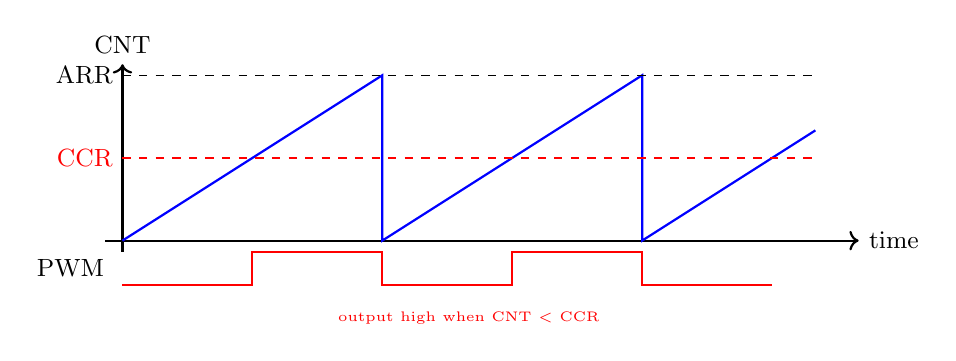
\begin{tikzpicture}[x=1.1cm, y=0.7cm]
  % Counter ramp
  \draw[thick, ->] (-0.2,0) -- (8.5,0) node[right]{\small time};
  \draw[thick, ->] (0,-0.2) -- (0,3.2) node[above]{\small CNT};
  % Sawtooth ramp
  \draw[thick, blue]
    (0,0) -- (3,3) -- (3,0) -- (6,3) -- (6,0) -- (8,2);
  % ARR line
  \draw[dashed] (0,3) node[left]{\small ARR} -- (8,3);
  % CCR line
  \draw[dashed, red] (0,1.5) node[left]{\small CCR} -- (8,1.5);
  % PWM output
  \draw[thick, red] (0,-0.8)
    -- ++(1.5,0) -- ++(0,0.6) -- ++(1.5,0) -- ++(0,-0.6)
    -- ++(1.5,0) -- ++(0,0.6) -- ++(1.5,0) -- ++(0,-0.6)
    -- ++(1.5,0);
  \node at (-0.6,-0.5) {\small PWM};
  \node[red] at (4,-1.4) {\tiny output high when CNT $<$ CCR};
\end{tikzpicture}
\caption{Timer up-count mode: counter ramps to ARR, resets; PWM output high while CNT $<$ CCR}
\end{figure}

\subsubsection{Sensor}

% ================================================================
\textbf{IMU: BNO055}

\textit{Communication protocol: I2C, address \texttt{0x28} (ADDR pin low) or \texttt{0x29} (ADDR pin high).
Bus speed up to 400\,kHz (Fast Mode). The MCU acts as master; BNO055 is slave.}

\medskip
\textit{Key registers:}

\begin{table}[H]
\centering
\begin{tabular}{llp{7cm}}
\hline
\textbf{Register} & \textbf{Address} & \textbf{Description} \\
\hline
\texttt{CHIP\_ID}       & \texttt{0x00} & Should read \texttt{0xA0} — used to verify communication \\
\texttt{OPR\_MODE}      & \texttt{0x3D} & Operation mode: \texttt{0x0C} = NDOF (full fusion), \texttt{0x00} = CONFIG \\
\texttt{PWR\_MODE}      & \texttt{0x3E} & Power mode: \texttt{0x00} = Normal \\
\texttt{SYS\_TRIGGER}   & \texttt{0x3F} & System trigger: \texttt{0x20} = reset \\
\texttt{UNIT\_SEL}      & \texttt{0x3B} & Unit selection: bit0=0 → degrees, bit0=1 → radians \\
\texttt{EUL\_H\_LSB}    & \texttt{0x1A} & Euler heading (yaw) LSB — 1 LSB = \(1/16\)° \\
\texttt{EUL\_H\_MSB}    & \texttt{0x1B} & Euler heading (yaw) MSB \\
\texttt{EUL\_P\_LSB}    & \texttt{0x1C} & Euler pitch LSB \\
\texttt{EUL\_P\_MSB}    & \texttt{0x1D} & Euler pitch MSB \\
\texttt{EUL\_R\_LSB}    & \texttt{0x1E} & Euler roll LSB \\
\texttt{EUL\_R\_MSB}    & \texttt{0x1F} & Euler roll MSB \\
\texttt{CALIB\_STAT}    & \texttt{0x35} & Calibration status: bits [7:6]=sys, [5:4]=gyro, [3:2]=accel, [1:0]=mag (3=fully calibrated) \\
\hline
\end{tabular}
\caption{BNO055 key registers}
\end{table}

\textit{Initialization \& data acquisition sequence:}

\begin{enumerate}
  \item \textbf{Power-on wait}: delay \(\geq\)650\,ms after power-up for internal oscillator to stabilize.
  \item \textbf{Verify chip}: read \texttt{CHIP\_ID} (0x00) → expect \texttt{0xA0}; retry up to 5 times if NACK.
  \item \textbf{Enter CONFIG mode}: write \texttt{0x00} to \texttt{OPR\_MODE} (0x3D); wait 19\,ms.
  \item \textbf{Set units}: write \texttt{UNIT\_SEL} (0x3B) → \texttt{0x00} (degrees, m/s², dps).
  \item \textbf{Set power mode}: write \texttt{0x00} (Normal) to \texttt{PWR\_MODE} (0x3E).
  \item \textbf{Set NDOF fusion mode}: write \texttt{0x0C} to \texttt{OPR\_MODE}; wait 7\,ms.
  \item \textbf{Read Euler angles} (burst read 6 bytes from \texttt{0x1A}):
  \begin{itemize}
    \item Combine LSB+MSB: \texttt{int16\_t raw = (MSB << 8) | LSB}
    \item Convert: \texttt{float degrees = raw / 16.0f}
    \item Order: \texttt{[EUL\_H, EUL\_P, EUL\_R]} → yaw, pitch, roll
  \end{itemize}
  \item \textbf{Repeat step 7} at desired rate (project uses 100\,Hz polling via TIM3 interrupt).
\end{enumerate}

\medskip

% ================================================================
\textbf{Encoder: AS5600}

\textit{Communication protocol: I2C, fixed address \texttt{0x36} (not configurable).
Bus speed up to 1\,MHz (Fast Mode Plus). Provides 12-bit absolute angle output.}

\medskip
\textit{Key registers:}

\begin{table}[H]
\centering
\begin{tabular}{llp{7.5cm}}
\hline
\textbf{Register} & \textbf{Address} & \textbf{Description} \\
\hline
\texttt{ZMCO}        & \texttt{0x00} & Number of times ZPOS/MPOS have been permanently written \\
\texttt{ZPOS\_H}     & \texttt{0x01} & Zero position (start angle) high byte [11:8] \\
\texttt{ZPOS\_L}     & \texttt{0x02} & Zero position (start angle) low byte [7:0] \\
\texttt{CONF\_H}     & \texttt{0x07} & Configuration high byte (slow filter, fast filter, watchdog) \\
\texttt{CONF\_L}     & \texttt{0x08} & Configuration low byte (power mode, hysteresis, output stage, PWM freq) \\
\texttt{RAW\_ANGLE\_H} & \texttt{0x0C} & Raw angle high byte [11:8] (before zero-position offset) \\
\texttt{RAW\_ANGLE\_L} & \texttt{0x0D} & Raw angle low byte [7:0] \\
\texttt{ANGLE\_H}    & \texttt{0x0E} & Processed angle high byte [11:8] (after zero offset, scaled to \texttt{MANG}) \\
\texttt{ANGLE\_L}    & \texttt{0x0F} & Processed angle low byte [7:0] \\
\texttt{STATUS}      & \texttt{0x0B} & bits [5:3]: MH=magnet too strong, ML=magnet too weak, MD=magnet detected \\
\texttt{AGC}         & \texttt{0x1A} & Automatic gain control value (0–255); nominal ~128 \\
\texttt{MAGNITUDE\_H}& \texttt{0x1B} & CORDIC magnitude high byte \\
\texttt{MAGNITUDE\_L}& \texttt{0x1C} & CORDIC magnitude low byte \\
\hline
\end{tabular}
\caption{AS5600 key registers}
\end{table}

\textit{Initialization \& data acquisition sequence:}

\begin{enumerate}
  \item \textbf{Verify magnet}: read \texttt{STATUS} (0x0B), check bit MD (bit 5) = 1 → magnet detected.
        If ML or MH set, reposition magnet until MD only.
  \item \textbf{Check AGC}: read \texttt{AGC} (0x1A); value should be 50–200 for reliable operation.
  \item \textbf{(Optional) Set zero position}: write current angle to \texttt{ZPOS\_H/L} to define the zero reference.
  \item \textbf{Read angle} (burst read 2 bytes from \texttt{0x0E}):
  \begin{itemize}
    \item \texttt{uint16\_t raw = ((ANGLE\_H \& 0x0F) << 8) | ANGLE\_L}
    \item Range: 0–4095 → 0°–360°
    \item Convert: \texttt{float deg = raw * 360.0f / 4096.0f}
  \end{itemize}
  \item \textbf{Compute RPM}: track angle over time, handle 0°/360° wrap-around,
        compute \(\Delta\theta / \Delta t\), convert to RPM.
  \item \textbf{Repeat step 4--5} at desired rate (project uses 1\,kHz via TIM3 interrupt).
\end{enumerate}

\subsubsection{Actuator}

\textbf{Steering: Angle 180 Servo}
\begin{itemize}
    \item \ldots
\end{itemize}

\textbf{Motivation: Brushless Motor \& ESC}
\begin{itemize}
    \item \ldots
\end{itemize}

% ------------------------------------------------------------
\subsection{Brain}

\subsubsection{Module Communication}

\textbf{Kernel}

\ldots

\textbf{Inter Process Communication}
\begin{itemize}
    \item Message Queue --- \ldots
    \item Unix Domain Socket --- \ldots
    \item TCP Socket --- \ldots
    \item Shared Memory --- \ldots
\end{itemize}

\textbf{Pub/Sub Model}
\begin{itemize}
    \item Node --- \ldots
    \item Topic --- \ldots
    \item Publish --- \ldots
    \item Subscribe --- \ldots
\end{itemize}

\textbf{Drop Policy}

\begin{itemize}
    \item Topic
    \item Message
    \item Payload
\end{itemize}

\textbf{C API / C++ Binding}

\textbf{Python Binding}

% ------------------------------------------------------------
\subsection{IO}

\begin{itemize}
    \item Serial Bridge
    \item Web Server / Web Socket
\end{itemize}

\subsubsection{Perception}

\textbf{Camera}
\begin{itemize}
    \item Input
    \item Output
    \item Algorithm
\end{itemize}

\textbf{Lane Detection}
\begin{itemize}
    \item Input
    \item Output
    \item Algorithm
\end{itemize}

\textbf{Object Detection}
\begin{itemize}
    \item Input
    \item Output
    \item Algorithm
\end{itemize}

\textbf{State}
\begin{itemize}
    \item Input
    \item Output
    \item Algorithm
\end{itemize}

\subsubsection{Localization}
\begin{itemize}
    \item Input
    \item Output
    \item Algorithm
\end{itemize}

\subsubsection{Planning}
\begin{itemize}
    \item Input
    \item Output
    \item Algorithm
\end{itemize}

\subsubsection{Control}
\begin{itemize}
    \item Input
    \item Output
    \item Algorithm
\end{itemize}

% ------------------------------------------------------------
\subsection{Monitor}

\begin{itemize}
    \item Web Server
    \item Dashboard
\end{itemize}

% ------------------------------------------------------------
\subsection{Simulation}

\begin{itemize}
    \item Visualization
    \item Direction Simulation
\end{itemize}

% ============================================================
\section{Source \& Description}

\end{document}